Для иллюстрации влияния микролинзирования на кривые блеска SN Refsdal использовался программный пакет {\tt{SNTD}} (\cite{pierelrodney2019}). Для области, в которой находится изображение S1 (см. Рис. \ref{fig:snrefsdalfig}) была построена карта микрокаустик со параметрами, найденными в предыдущем разделе. Сверхновая моделировалась кругом с постоянной поверхностной яркостью, который расширяется со скоростью v=15000 км/с в течение 200 дней (значения скорости расширения и периода наблюдения выбраны несколько произвольно с целью проиллюстрировать эффект). В зависимости от положения источника на карте микрокаустик можно наблюдать различные “шумы” от микролинзирования (см. Рис. \ref{fig:sntd_example}).

\begin{figure}[H]
    \centering
	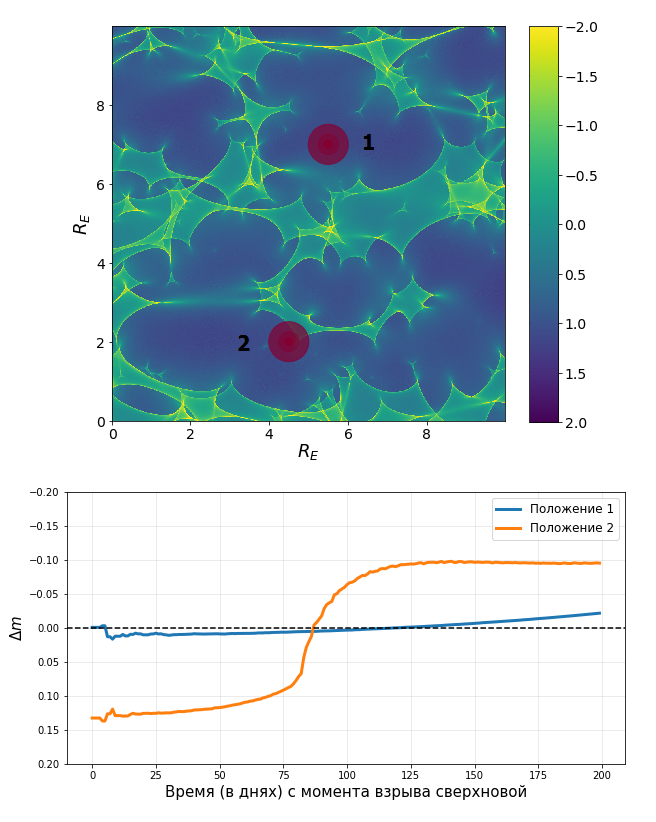
\includegraphics[scale=0.75]{pics/sntd_example.png}
	\caption{\textit{Сверху}: карта микрокаустик для изображения S1 сверхновой Refsdal, цветовая шкала представлена в единицах звёздных величин. Жёлтый цвет соответствует усилению, фиолетовый - ослаблению. \textit{Снизу}: вклад $\Delta m$ (в единицах звёздных величин), обусловленный микролинзированием, в зависимости от времени с момента начала расширения сверхновой, для двух различных положений источников. \label{fig:sntd_example}} 
\end{figure}

Для положения 1 источника, который находится в области с равномерным усилением и не пересекает каустики, вклад от микролинзирования слабый и примерно постоянный во времени. Напротив, в положении 2 источник при расширении захватывает области сильного усиления, что может заметно повлиять на форму истинной кривой блеска источника (флуктуации ~0.3 звездных величин). 